\section{System Design}

\begin{figure}[!hb]   %% START_FIGURE
\centerline{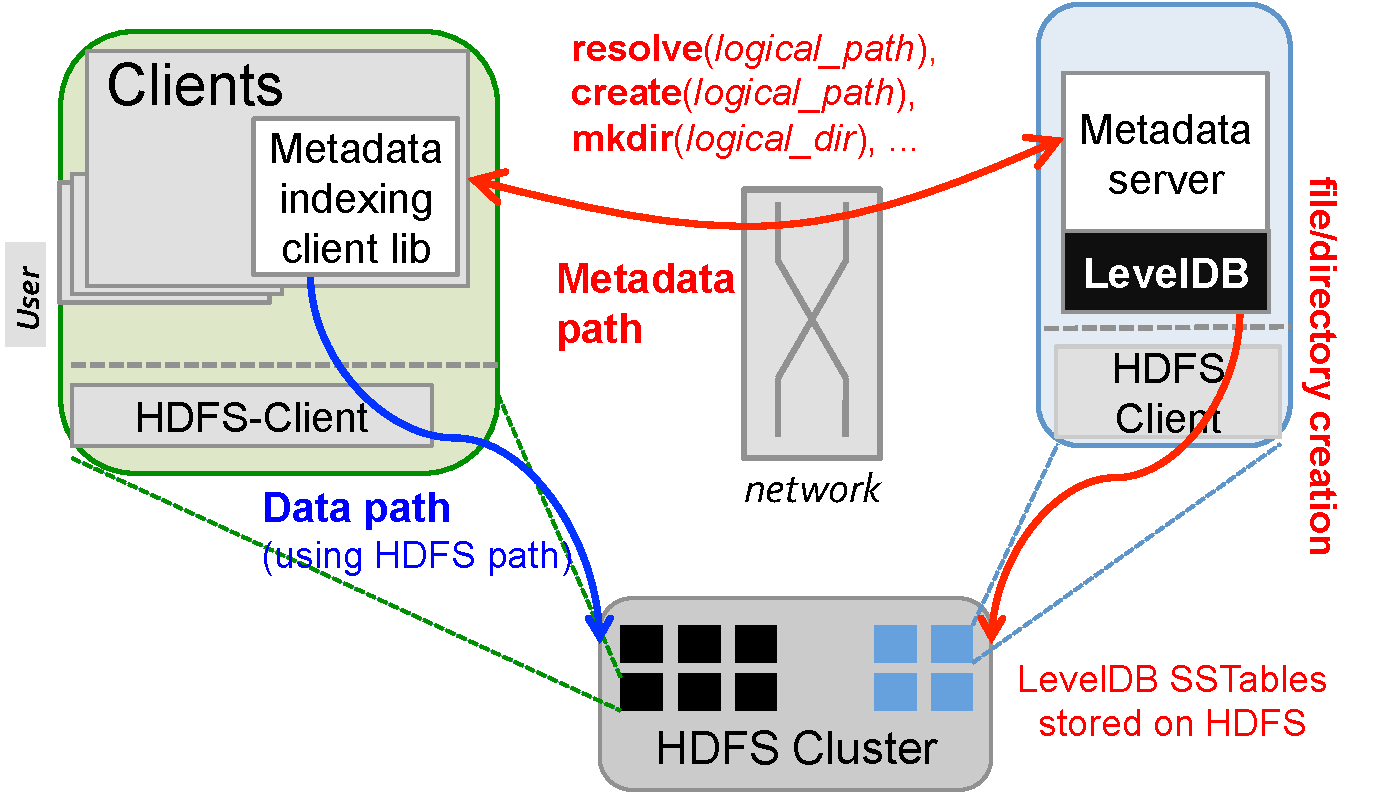
\includegraphics[scale=0.35]{./figs/giga-impl-leveldb-clusterfs}}
\vspace{10pt}
\caption{\textit{\footnotesize
Our scalable metadata service integrates two components: GIGA+ \cite{GIGA11},
a highly parallel and load-balanced indexing technique 
to partition metadata over multiple servers, and TableFS \cite{TableFS},
an log-structured (LevelDB) on-disk metadata representation on each server.
This integrated solution is layered on top of an existing cluster
file system deployment (PanFS) to improve metadata
and small file operation efficiency.
}}
%\vspace{10pt}
\hrule
\label{fig:design}
\end{figure}       %% END_FIGURE

Figure \ref{fig:design} presents the overall architecture of our scalable
metadata service. Our metadata service is a middleware inserted into
existing deployments of cluster file systems to improve metadata efficiency
while maintaining high I/O bandwidth for data transfers.
The system uses a client-server architecture,
and consists of three core components:

\begin{itemize}
\item{\textbf{Client:}} Applications interact with our middleware
through the FUSE user-level file system \cite{fuse},
through a library directly linked into the application
or through a module in a common library such as MPI-IO \cite{mpi}.
The stateless client-side code redirects applications' file operations
to the appropriate destination according to the types of operations.
All metadata requests (e.g. \texttt{create()} and \texttt{mkdir()}),
and data requests on small files (e.g. \texttt{read()} and \texttt{write()}),
are handled by the metadata indexing modules that address
these requests to the appropriate server.
For all data operations on large size files, the client code redirects
the request directly to the underlying cluster file system to take full
advantage of data I/O bandwidth. A newly created, but growing file
may be transparently reopened by the client module.

\item{\textbf{Metadata Indexing Server:}}
Each indexing server manages its local metadata storage backend to store and
access all metadata information and small file data.
It uses the GIGA+ algorithm to
partition large directories across indexing servers. It also monitors the growth
of small files, and migrates newly large files into
the underlying cluster file system
when its size exceeds a threshold.

\item{\textbf{Metadata Storage Backend:}}
The metadata storage backend is a modified version of \tfs which packs metadata
and small file data into large, log-structured, flat files,
and stores these files
in the underlying cluster file system. Since \tfs converts random updates into
sequential writes, it greatly improves disk performance. In order to
dynamically redistribute large directories,
the metadata storage backend also modifies
\tfs to support exporting and importing flat files in batch.

\end{itemize}

Remainder of this section describes more details of our system.
Section \ref{design.giga} presents a primer on how \giga distributes metadata.
Section \ref{design.tablefs} shows how \tfs stores all file system metadata
and small files using a single on-disk structure on each server.
Section \ref{design.integration} focus on the challenges in effectively
integrating \giga and \tfs to work with existing cluster file systems.

\subsection{Metadata Storage Backend}
\label{design.tablefs}

To effectively build \sys middleware that integrates
the \giga distribution mechanism and the \tfs metadata representation,
we have to tackle two main challenges:
modify \tfs to support for
migrating directory partitions as required by \giga;
and decouple metadata and data paths to
achieve high performance for both paths.
This section discusses the modifications we made to
overcome these two challenges.


~\\
\textbf{Metadata representation -- }
\tfs stores all additional metadata including \giga per-directory hash
partitions, entries in each hash partition, and \giga
bootstrapping information such as root partition entry
and \giga configuration state.
The general schema used to store all metadata is:

\begin{table}[!htc]
\center
\vspace{10pt}
\begin{tabular}{c|c}
key & \texttt{parentDirID,gigaPartitionID,hash(dirEntry)} \\
\midrule \\
value & \texttt{attributes,[symlink|data|gigaMetaState]} \\
\end{tabular}
\label{tab:keyschema}
\end{table}

The main difference from the \tfs schema described in Section
\ref{design.tablefs} is the addition of two \giga specific fields:
\texttt{gigaPartitionID} to identify a
\giga hash partition within a directory and \texttt{gigaMetaState} to store the
hash partition related mapping information for directories.
These \giga related fields are used only
if a large directory is large enough to be
distributed over multiple metadata servers.
\footnote{A optimization is to eliminate \texttt{gigaPartitionID} in the key
by using the same hash function for both \giga and \tfs keys,
since the hash of entry name can determine the partition ID.}

~\\
\textbf{Partition splitting -- }
Each server's \tfs instance stores metadata,
including \giga directory partitions and their directory
entries in \ldb which stores them as
a set of files (whose format is called SSTable) in a server specific directory
in the underlying cluster file system.
Each \giga server process splits a large partition $P$ on
into itself and another hash partition $P'$ which is managed by a
different server; this split involves migrating approximately half the entries
from old partition $P$ to the new partition $P'$ on another server.
During splitting, the partition in migration is locked against client
for simplification. We explored several ways
to perform this cross-server partition split.

A straightforward solution would be to perform a range scan on
partition $P$, and remove about half the entries
(that will be migrated to the new partition $P'$) from $P$.
All removed entries would then be batched together
and sent in a large RPC message to the server that will manage partition $P'$.
The split receiver would insert each key in the batch into its own \tfs instance.
While simplicity of this solution makes it attractive,
it is slow in practice and vulnerable to failures during splitting.

We have devised a faster and safer technique to
reduce the time that the splitting range is locked.
The immutability of SSTables in \ldb makes a fast bulk insert possible --
an SSTable whose range does not overlap any part of a current LSM tree
can be added to Level 0 without its data being pushed through the
write-ahead log and minor compaction process.
To take advantage of this opportunity, we extended \tfs
to support a three-phase \giga split operation:

\begin{itemize}
\item{Phase 1:} The split initiator locks and
then performs a range scan on its \tfs instance
to find all entries in the hash-range that needs to be moved to another server.
Instead of packing these into an RPC message,
the results of this scan are written in SSTable format to a file in the
underlying cluster file system.

\item{Phase 2:} The split initiator notifies the split receiver about
the path to the SSTable-format split file in a much smaller RPC message.
Since this file is stored in shared storage,
the split receiver directly inserts this file as a symbolic link
into the \ldb tree structure without actually copying this file.
The insertion of this file into the split receiver is the commit
part of the split transaction.

\item{Phase 3:} The final step is a clean-up phase:
after the split receiver completes the bulk insert operation, it notifies the
initiator, who then deletes the migrated key-range from its \tfs instance
and unlocks the range.
\footnote{The three phases of splitting can be refined even further:
Assume that the splitting is initiated at the time $T_{split}$.
The split initiator can generate SSTables containing entries
older than $T_{split}$ without locking the hash range.
When the generation of SSTables with entries older than $T_{split}$ is finished,
the split initiator can lock the hash range and then write SSTables with
newly added or updated entries later than $T_{split}$.
By doing so, the duration of locking splitting hash range can be further reduced.
However, due to the code complexity of this optimization,
we left this optimization for future work.}

\end{itemize}

\subsection{Transaction Support}


\subsection{Decoupled Data and Metadata Path}


\subsection{Fault Tolerance}

